
\section{Theory}

This section provides a short introduction to relevant theory in orbital mechanics and propagation of uncertainties. The intended reader is someone with a technical background other than orbital mechanics or statistics, and the goal is to give a sufficient understanding of necessary concepts. 


\subsection{Orbital Mechanics}

The sections on orbital mechanics are mostly based on the book by Curtis \cite{Curtis2009}.



\subsubsection{Orbital Parameters}

The following is an introduction to a parametric description of orbits, using the definitions from Curtis \cite{Curtis2009}. Under the assumption that an orbit is an ideal Keplerian orbit, it can be uniquely identified using six orbital elements. Three parameters are required to define the orbit on a plane, and three additional parameters are needed to further place the orbit in three dimensional space. \\

The three parameters used to describe an orbit on a plane are the \textit{specific angular momentum}, \textit{eccentricity}, and \textit{true anomaly}. The specific angular momentum is, as the name suggests, the angular momentum of the orbiting object. This value is constant everywhere on a given orbit. The eccentricity value describes how much the shape of the orbit deviates from a circle, and can be found by dividing the distance between the center of the orbit and one of the foci by the \textit{semi-major axis} (longest distance between the orbit and the central body). The shape of an orbit corresponding to different eccentricity values is given in Table \ref{table:eccentricity}. The true anomaly is the angle as seen from the center of the orbit between the position of the orbiting object and \textit{periapsis} (the shortest distance to the central body). \\

\begin{table}[h]
\centering
\begin{tabular}{@{}ll@{}}
\toprule
$e = 0$      & Circle    \\
$0 < e < 1 $ & Ellipse   \\
$e = 1$      & Parabola  \\
$e > 1 $     & Hyperbola \\
\bottomrule
\end{tabular}
\caption{Orbital shapes for different eccentricity values}
\label{table:eccentricity}
\end{table}


To place the orbit in three dimensional space, three axis rotations are additionally required. The orbital elements corresponding to these rotations are the \textit{inclination}, \textit{right ascension of the ascending node} and the \textit{argument of perigee}. The inclination describes the angle between the orbital plane and the \textit{equatorial} (Earth XY) plane. The right ascension of the ascending node is the angle between the equatorial X-axis and the point on the equatorial plane where the orbit passes through from below. The third angle, argument of perigee, is the angle in the orbital plane between the point the orbit passes through the equatorial plane from below and the point of perigee on the orbit. \\


A summary of the six orbital elements is given in Table \ref{table:orbital_parameters}. \\


\begin{table}[h]
\centering
\begin{tabular}{@{}llll@{}}
\toprule
%\multicolumn{4}{c}{Orbital Parameters}                            \\ \midrule
Name                                  & Symbol              & Range     & Unit \\ \midrule
Specific angular momentum             & \textit{h}          & -         & $\frac{kgm}{s^2}$ \\
Inclination                           & \textit{i}          & [0, 180]  & Deg    \\
Right ascension of the ascending node & $\mathit{\Omega}$   & [0, 360]  & Deg  \\
Eccentricity                          & \textit{e}          & -         & -    \\
Argument of perigee                   & $\mathit{\omega}$   & [0, 360]  & Deg  \\
True anomaly                          & $\mathit{\Theta}$   & [0, 360]  & Deg  \\ \bottomrule
\end{tabular}
\caption{Overview of the six orbital parameters}
\label{table:orbital_parameters}
\end{table}







\subsubsection{Keplerian Orbit}

A Keplerian orbit assumes that all forces acting on the system, consisting of orbiting object and central body, are generated by the two point masses. Kepletian orbits are thus said to be a special case of the two-body motion problem. The fundamental equation of relative two-body motion is presented in Eq. \ref{eq:relative_twobody_motion}, in which $\mu = G(m_1 + m_2)$ is the gravitational parameter with unit $km^3s^{-2}$. \\

\begin{equation}
    \Ddot{\mathbf{r}} = - \frac{\mu}{r^3} \mathbf{r}
    \label{eq:relative_twobody_motion}
\end{equation}{}


The mathematical description of a Keplerian orbit relative to the central body are various conic sections, i.e. ellipses, parabolas or hyperbolas. \\


\todo{Fill in Kepler's orbital equations}

\todo{Define the Universal Parameter description of Keplerian orbits}




\subsubsection{Coordinate Systems}


\paragraph{Earth Centered Intertial Coordinate System} 

Define the Earth Centered Intertial (ECI) coordinate frame. \\
\todo{Fill in}



\paragraph{Perifocal Coordinate System} 
The center of the perifocal coordinate system is at the focus of the orbit. The perifocal frame is defined with the unit vectors $\hat{\mathbf{p}}$, $\hat{\mathbf{q}}$ and $\hat{\mathbf{w}}$. The unit vectors $\hat{\mathbf{p}}$ and $\hat{\mathbf{q}}$ lie in the orbital plane, with $\hat{\mathbf{p}}$ pointing towards the \textit{periapsis} of the orbit and $\hat{\mathbf{q}}$ towards the point at which \textit{true anomaly} is equal to $90 \deg$. The unit vector $\hat{\mathbf{w}}$ is the cross product of the unit vectors in the orbital plane, $\hat{\mathbf{w}} = \hat{\mathbf{p}} \times \hat{\mathbf{q}}$, and thus points in the same direction as the angular momentum vector $\Vec{\mathbf{h}}$ of the orbiting object. \\

The position of the orbiting object described in the perifocal plane is given in Eq. \ref{eq:radius_perifocal_frame}, and velocity in Eq. \ref{eq:velocity_perifocal_frame}.

\begin{equation}
    \Vec{\mathbf{r}} = \Bar{x}\hat{\mathbf{p}} + \Bar{y}\hat{\mathbf{q}}
    \label{eq:radius_perifocal_frame}
\end{equation}

\begin{equation}
    \Vec{\mathbf{v}} = \dot{\Vec{\mathbf{r}}} = \dot{\Bar{x}}\hat{\mathbf{p}} + \dot{\Bar{y}}\hat{\mathbf{q}}
    \label{eq:velocity_perifocal_frame}
\end{equation}


\paragraph{Local Vertical Local Horizontal Coordinate System} 

Define the Local Vertical Local Horizontal (LVLH) coordinate frame. \\  
\todo{Fill in}






\subsubsection{Orbital Perturbations}

Orbital perturbations are effects that cause an object's orbit to deviate from an ideal Keplerian orbit.\\


Sources of uncertainty in orbital mechanics will be introduced in the following section. Uncertainties in orbital estimations can originate from phenomena in the physical world, or come from approximations and deviations in the models used.  \\

Based on the review by Luo and Yang \cite{luo_review_2017}, who follow the opinion of Fehse \cite{2003ARaD}, the uncertainties related to space operation can be divided into three categories: \textit{Dynamic model errors}, \textit{actuation errors} and \textit{navigation errors}. Dynamic model errors concern the deviations in the model parameters to the real world values, such as the gravitational parameters, drag and radiation pressure. Actuation errors concern the difference between the correct actuation values and the values produced by the actuators and control system. Navigation errors are the deviations in the perceived state of the system from the actual state. An overview of the types of uncertainty in orbital mechanics is given in Table \ref{table:error_sources}.\\



\begin{table}[h!]
\centering
\begin{tabular}{@{}ll@{}}
\toprule
\textbf{Classification}                        & \textbf{Parameter}           \\ \midrule
\multirow{3}{*}{Dynamic Model Errors} & Gravitational Field \\
                                      & Drag                \\
                                      & Radiation Pressure  \\ \midrule
\multirow{3}{*}{Actuation Errors}     & Direction           \\
                                      & Timing              \\
                                      & Force               \\ \midrule
\multirow{3}{*}{Navigation Errors}    & Atmospheric Effects \\
                                      & Instrument Modeling \\
                                      & Clock Accuracy   \\    
\bottomrule
\end{tabular}%
\caption{Error Sources in Orbital Mechanics}
\label{table:error_sources}
\end{table}
    




\paragraph{Earth's Oblateness}

The Earth's equatorial radius is larger than the polar radius due to the centrifugal forces of its spin.  \textit{Oblateness} is a measure of the flattening of a sphere, and is defined as follows:

$$ \text{Oblateness} = \frac{\text{Equatorial radius - Polar radius}}{\text{Equatorial radius}} $$


An oblate spheroid has a gravitational field that varies with latitude. The \textit{second zonal harmonic}, $\mathbf{J_2}$, is a parameter that quantifies the effects of oblateness on gravitational pull. 


\begin{equation}
    \mathbf{a} = \frac{3 \mu J_2 R_e^2}{2 r^5} \left( \frac{5 z^2}{r^2} \begin{bmatrix} 1 \\ 1 \\ 1 \end{bmatrix} - \begin{bmatrix} 1 \\ 1 \\ 3 \end{bmatrix} \right) \mathbf{p}
\end{equation}{}


\paragraph{Atmospheric Drag}

Objects orbiting near Earth will have a negative acceleration due to collisions with atmospheric particles, known as drag. The magnitude of the acceleration is dependent on the density of the atmospheric particles. The density of the atmosphere has both latitudinal, longitudinal, periodic and random variations, but is mainly dependent on the gravitational forces exerted by the Earth, and thus the altitude of the orbit. Other contributing factors to the atmospheric density are the sun's position and radiation activity, and variations in Earth's magnetic field. \\

\todo{Exponential Atmospheric Model}

\begin{equation}
    \mathbf{a} = - \frac{1}{2} \frac{C_D S}{M} \rho \mathbf{v_{rel}} \left( \mathbf{v} + \begin{bmatrix} 0 & \omega_e & 0 \\ -\omega_e & 0 & 0 \\ 0 & 0 & 0 \end{bmatrix} \mathbf{p} \right)
\end{equation}{}


\paragraph{Thruster Dynamics}


\subsubsection{Lagrange Coefficients}

Using the Lagrange Coefficients, \textit{f} and \textit{g}, from the French mathematical physicist Joseph-Louis Lagrange (1736-1813), we are able to describe the position and velocity of an orbiting object at any point in time if the initial conditions are known. This is shown in Eq. \ref{eq:radius_lagrange_coefficients}. 
\todo{Does this assume Keplerian motion??}


\begin{equation}
    \Vec{\mathbf{r}} = f \Vec{\mathbf{r_0}} + g \Vec{\mathbf{v_0}}
    \label{eq:radius_lagrange_coefficients}
\end{equation}

The Lagrange Coefficients $f$ and $g$, and their time derivatives $\dot{f}$ and $\dot{g}$, are defined below.

\begin{align}
    f &= \frac{ \Bar{x} \dot{\Bar{y_0}} - \Bar{y} \dot{\Bar{x_0}} }{ h }
    \label{eq:lagrange_f} \\
    g &= \frac{ - \Bar{x} \Bar{y_0} + \Bar{y} \Bar{x_0} }{ h } 
    \label{eq:lagrange_g} \\
    \dot{f} &= \frac{ \dot{\Bar{x}} \dot{\Bar{y_0}} - \dot{\Bar{y}} \dot{\Bar{x_0}} }{ h } 
    \label{eq:lagrange_f_dot} \\
    \dot{g} &= \frac{ - \dot{\Bar{x}} \Bar{y_0} + \dot{\Bar{y}} \Bar{x_0} }{ h } 
    \label{eq:lagrange_g_dot}
\end{align}

Using the change in true anomaly $\Delta \Theta$, or the change in universal anomaly $\chi$, the Lagrange Coefficients and their time derivatives have the following expressions. The left column in the functions below are the expressions based on true anomaly $\Delta \Theta$, and the right column are the expressions based on universal anomaly $\chi$.

\begin{align}
    f &= 1 - \frac{ \mu r }{ h^2 } \left( 1 - \cos{\Delta \Theta} \right) &&= 1 - \frac{\chi^2}{r} C\left(z\right)
    \label{eq:lagrange_anomaly_f} \\
    g  &= \frac{ r_0 r }{ h } \sin{\Delta \Theta} &&= \Delta t - \frac{1}{\sqrt{\mu} \chi^3 S\left( z \right)}
    \label{eq:lagrange_anomaly_g} \\
    \dot{f} &= \frac{\mu}{h} \frac{1 - \cos{\Delta \Theta}}{\sin{\Delta \Theta}} \left[ \frac{\mu}{h^2} \left(1 - \cos{\Delta \Theta} \right) - \frac{1}{r_0} - \frac{1}{r} \right] &&= \frac{\sqrt{\mu}}{r_0 r} \chi \left[z S\left( z \right) - 1 \right]
    \label{eq:lagrange_anomaly_f_dot} \\
    \dot{g} &= 1 - \frac{\mu r_0}{h^2} \left(1 - \cos{\Delta \Theta} \right) &&= 1 - \frac{\chi^2}{r} C\left( z \right)
    \label{eq:lagrange_anomaly_g_dot}
\end{align}

For the functions above, $\alpha = \frac{1}{a}$ is the inverse of the semimajor axis, $z = \alpha \chi^2$, and $C(z)$ and $S(z)$ are \textit{Stumpff functions} defined below.

\begin{align}
    C(z) &= \sum_{k = 0}^{\infty} (-1)^k \frac{z^k}{(2k + 2)!} \\
    S(z) &= \sum_{k = 0}^{\infty} (-1)^k \frac{z^k}{(2k + 3)!}
\end{align}{}




\subsubsection{Lambert's problem}

Lambert's problem, from the French-born German astronomer J. H. Lambert (1728-1777), concerns finding the trajectory joining two orbital points $P_0$ and $P$, given the transfer time $\Delta t$.  \\

Algorithm \ref{algo:lambert} presents an approach using the Lagrange Coefficients and the conservation of angular momentum to solve Lambert's problem. The method presented is based on \textit{Algorithm 5.2} from the book by Curtis \cite{Curtis2009}.

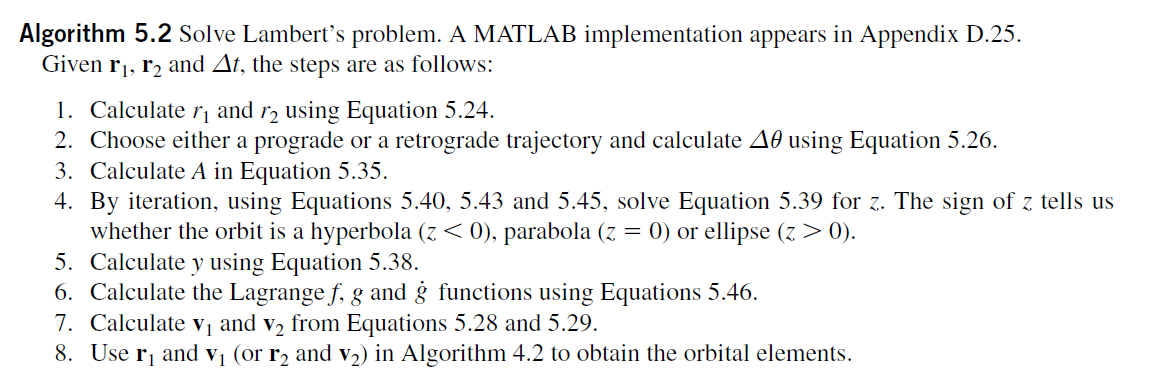
\includegraphics[width=\textwidth]{Images/Alg52.PNG}

\begin{algorithm}
    \setstretch{1.2}
    \DontPrintSemicolon
    \KwIn{Starting point, end point, direction and time frame of desired trajectory}
    \KwOut{Initial velocity required to follow desired trajectory and velocity at end point}
    Calculate the change in true anomaly, $\mathit{\Delta\Theta}$, based on starting point, end point and direction of orbit (prograde or retrograde)\;
    \Return{velocityStart, velocityEnd}\;
    \caption{Solve Lambert's Problem Using Lagrange Coefficients}
    \label{algo:lambert}
\end{algorithm}

\todo{Insert Algorithm from Curtis}

\todo{Expand on the various optimal solutions, time energy etc.}

%%%%%%%%%%%%%%%%%%%%%%%%%%%%%%%%%%%%%%%%%%%%%%%%%%%%%%%%%%%%%%%%


\subsection{Uncertainty Propagation}

In the following section different methods of uncertainty propagation are presented. The term \textit{uncertainty propagation} refers to the method of predicting a systems state and associated uncertainty at a certain point in time, given information about the initial state and uncertainty of the system. A propagator can be either linear or nonlinear, with several approaches existing within both classes. \\


\subsubsection{Monte Carlo Simulations}

Monte Carlo simulation relies on repeated random sampling to obtain numerical results. MC simulation is computationally heavy, but has the advantage that when the number of samples approaches infinity, the result converges towards the true probability distribution of the system. \\


